\documentclass[a4paper]{article}
\usepackage[spanish]{babel}
\usepackage[utf8]{inputenc}
\usepackage{graphicx}
\usepackage{enumerate}
\usepackage{listings}
\usepackage{color}
\usepackage{indentfirst}
\usepackage{fancyhdr}
\usepackage{latexsym}
\usepackage{blkarray}
\usepackage{multirow}
\usepackage[colorlinks=true, linkcolor=black]{hyperref}
%\usepackage{makeidx}
%\usepackage{float}
\usepackage{calc}
\usepackage{amsmath, amsthm, amssymb}
\usepackage{amsfonts}
%\lstset{language=C}
\definecolor{gray}{gray}{0.5}
\definecolor{light-gray}{gray}{0.95}
\definecolor{orange}{rgb}{1,0.5,0}

\usepackage{fancyhdr}
\pagestyle{fancy}

%\renewcommand{\chaptermark}[1]{\markboth{#1}{}}
\renewcommand{\sectionmark}[1]{\markright{\thesection\ - #1}}

\fancyhf{}

\fancyhead[LO]{Sección \rightmark} % \thesection\
\fancyfoot[RO]{\thepage}
\renewcommand{\headrulewidth}{0.5pt}
\renewcommand{\footrulewidth}{0.5pt}
\setlength{\hoffset}{-0.8in}
\setlength{\textwidth}{16cm}
%\setlength{\hoffset}{-1.1cm}
%\setlength{\textwidth}{16cm}
\setlength{\headsep}{0.5cm}
\setlength{\textheight}{25cm}
\setlength{\voffset}{-0.7in}
\setlength{\headwidth}{\textwidth}
\setlength{\headheight}{13.1pt}

\renewcommand{\baselinestretch}{1.1}  % line spacing


% \setcounter{secnumdepth}{2}
\usepackage{underscore}
\usepackage{caratula}
\usepackage{url}
\usepackage{float}

\usepackage{commath}
\usepackage[draft]{todonotes}
\usepackage{caption}

\usepackage{algorithm}
\usepackage[noend]{algpseudocode}
\usepackage{array}
\usepackage{xcolor,colortbl}
\usepackage{amsthm}
\usepackage{mathtools}
\usepackage{listings}
\usepackage{svg}
\usepackage{systeme}
\usepackage{color,soul}

\captionsetup[figure]{labelformat=empty}% redefines the caption setup of the figures environment in the beamer class.
\makeatletter
\renewcommand*\env@matrix[1][*\c@MaxMatrixCols c]{%
  \hskip -\arraycolsep
  \let\@ifnextchar\new@ifnextchar
  \array{#1}}
\makeatother


\newcommand{\cod}[1]{{\tt #1}}
\newcommand{\negro}[1]{{\bf #1}}
\newcommand{\ital}[1]{{\em #1}}
\newcommand{\may}[1]{{\sc #1}}
\newcommand{\tab}{\hspace*{2em}}

\hypersetup{
 pdfstartview= {FitH \hypercalcbp{\paperheight-\topmargin-1in-\headheight}},
 pdfauthor={Grupo},
 pdfsubject={Dise\~{n}o}
}

\lstdefinestyle{customc}{
  backgroundcolor=\color{light-gray},
  belowcaptionskip=1\baselineskip,
  breaklines=true,
  numbers=left,
  xleftmargin=\parindent,
  language=C,
  showstringspaces=false,
  basicstyle=\footnotesize\ttfamily,
  keywordstyle=\bfseries\color{blue},
  commentstyle=\itshape\color{gray},
  identifierstyle=\color{black},
  stringstyle=\color{orange},
}

\lstdefinestyle{customasm}{
  backgroundcolor=\color{light-gray},
  belowcaptionskip=1\baselineskip,
  numbers=left,
  xleftmargin=\parindent,
  language=[x86masm]Assembler,
  keywordstyle=\bfseries\color{blue},
  basicstyle=\footnotesize\ttfamily,
  commentstyle=\itshape\color{gray},
}

\lstset{escapechar=@}


\begin{document}

\thispagestyle{empty}
\materia{Métodos Númericos}
\submateria{2do Cuatrimestre - 2017}
\titulo{Trabajo Práctico I}
% \subtitulo{Subtitulo}
\integrante{Jonathan Seijo}{592/15}{jon.seijo@gmail.com}
\integrante{Lucas De Bortoli}{736/15}{lu_cas_.97@hotmail.com.ar}
\integrante{COMPLETAR}{COMPLETAR}{COMPLETAR}
\integrante{COMPLETAR}{COMPLETAR}{COMPLETAR}

\makeatletter

\maketitle
\newpage

\thispagestyle{empty}
\vfill

\thispagestyle{empty}
\vspace{3cm}
\tableofcontents
\newpage

\newenvironment{myindentpar}[1]
{\begin{list}{1}
         {\setlength{\leftmargin}{#1}}
         \item[]
}
{\end{list} }

%\normalsize
\newpage

% -------------------------------------------------------
% Introducción Teórica
% -------------------------------------------------------
\section{Introducción}

% Pautas de tp hablan de "brave introduccion"

Este trabajo consiste en la digitalización de objetos 3D basándose en imágenes producidas con cámaras tradicionales, utilizando la técnica de \textit{fotometría estéreo}. Mostraremos que utilizando luces provenientes de diferentes ángulos, podemos aproximar las normales a la superficie y estimar las profundidades de cada punto.

Para esto debemos resolver varios sistemas de ecuaciones lineales, los cuáles resolveremos algorítmicamente de forma matricial. Usaremos en un primer caso el método clásico de Eliminación Gaussiana, y veremos como utilizando factorización LU podemos reducir los tiempos de cómputo. Luego, utilizaremos la factorización de Cholesky.

Los experimentos .... []
\todo[inline]{Completar breve pantallazo a experimentos}

% -------------------------------------------------------
% Calibracion
% -------------------------------------------------------
\newpage

% Template de matriz
% \[
% \begin{bmatrix} % Matriz con linea rectangular
% \begin{pmatrix} % Matriz con linea redonda
%     x_{11} & x_{12} & x_{13} & \dots  & x_{1n} \\
%     x_{21} & x_{22} & x_{23} & \dots  & x_{2n} \\
%     \vdots & \vdots & \vdots & \ddots & \vdots \\
%     x_{d1} & x_{d2} & x_{d3} & \dots  & x_{dn}
% \end{pmatrix}
% \end{bmatrix}
% \]

\section{Calibración}

El paso anterior al cálculo de las profundidades es el cálculo de los vectores normales a todo punto de la superficie. Para esto, se eligen tres luces diferentes (por ejemplo si elegimos 1, 2 y 3, nuestros vectores luz serán $s^{1}$, $s^{2}$ y $s^{3}$ respectivamente) y utilizando las intensidades ya registradas ($I_i$) queremos encontrar los $m$ que son solución, donde $m$ es un vector que depende del vector normal y de una constante del objeto. Cabe aclarar que el sistema se deberá resolver para cada píxel de la imagen, por lo que ya conocemos las intensidades del píxel dado para toda imagen. Nos encontramos entonces con el primer problema, porque los vectores de luz no son un dato conocido. \\

El sistema que queremos resolver es el siguiente: \\

\[
% \begin{bmatrix} % Matriz con linea rectangular
\begin{pmatrix}
    s_{x}^{1} & s_{y}^{1} & s_{z}^{1} \\
    s_{x}^{2} & s_{y}^{2} & s_{z}^{2} \\
    s_{x}^{3} & s_{y}^{3} & s_{z}^{3}
\end{pmatrix}
% \end{bmatrix}
\begin{pmatrix}
    m_{x} \\
    m_{y} \\
    m_{z}
\end{pmatrix}
=
\begin{pmatrix}
    I_{1} \\
    I_{2} \\
    I_{3}
\end{pmatrix}
\]

Pero no conocemos los $s_{j}^{i}$. \\

Tenemos que $S = (s_{x}^{i}, s_{y}^{i}, s_{z}^{i})$ es el vector luz en la imagen $i$. Dado que vamos a explicar el cálculo para una imagen cualquiera, omitiremos el supraíndice $i$ para una notación más relajada.

Llamemos $c = (c_{x}, c_{y}, c_{z})$ al centro de la esfera. Pensemos la luz como un vector que apunta hacia el centro. El vector $S$ toca la superficie en un cierto punto $p = (p_{x}, p_{y}, p_{z})$, pero $p$ no es un punto al azar, sino que es el punto más iluminado de la esfera. Por lo tanto, la dirección de luz que nos interesa es $S =  c - p$.\\

{\centering
    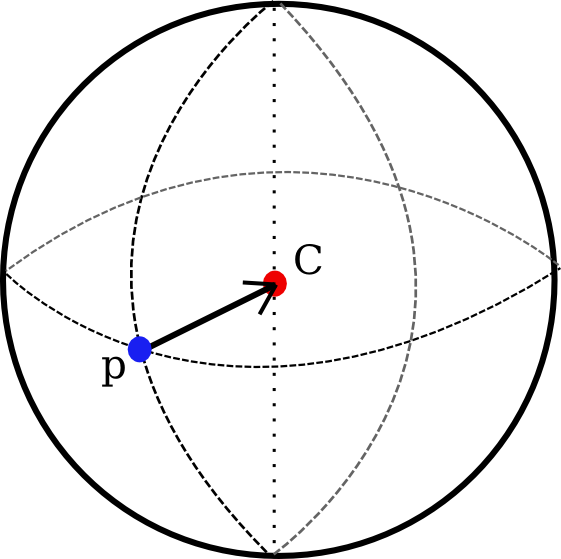
\includegraphics[scale=0.9]{informe/imagenes/esfera/esferaModelo.png} \\
    \captionof{figure}{Imagen del vector que nos interesa, $S = c - p$}
}

$ $\newline

Más precisamente, $S = (c_{x} - p_{x}, c_{y} - p_{y}, c_{z} - p_{z}).$ En principio no conocemos ninguno de estos valores, pero concentrémonos en calcular sobre el eje $x$ e $y$. De la imagen de la esfera (2D) podemos conocer algunos datos. En la implementación utilizamos la máscara provista por la cátedra para simplificar los cálculos. \\

Como los píxeles en la máscara son blancos o negros, es muy sencillo identificar los puntos que pertenecen a la esfera con sólo ver su color. Recorriendo todos los puntos y tomando máximos y mínimos obtenemos 4 puntos clave: El punto del círculo que está más arriba $A$, el más abajo $A'$, el de más a la izquierda $B$ y el de más a la derecha $B'$. \\

{\centering
    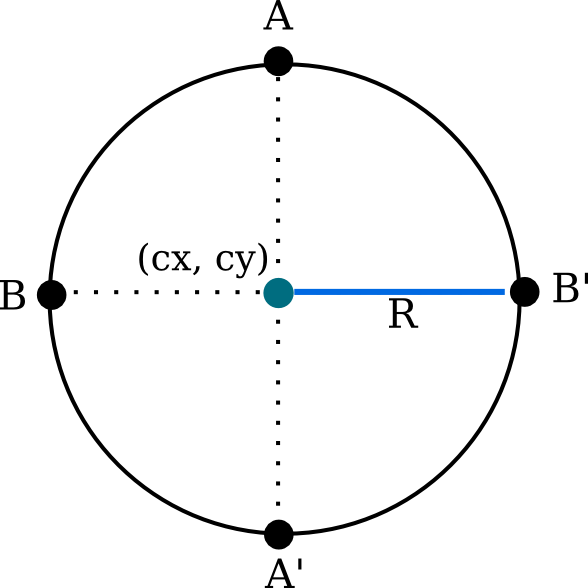
\includegraphics[scale=0.5]{informe/imagenes/esfera/circulo.png} \\
}

Puede verse fácilmente que el radio $R$ del círculo es la mitad de la distancia entre $B$ y $B'$

\begin{center}
$R = \frac{|B'_x - B_x|}{2}$.
\end{center}

Además, sabiendo que $c$ es el centro del círculo,

\begin{center}
    $c_{x} = B_x + R$ \\
    $c_{y} = A_y + R$
\end{center}

Necesitamos encontrar también quién es $p$. Una primera idea fue recorrer todos los píxeles y quedarnos con el de mayor intensidad. Esto nos trajo problemas pues en una imagen no hay un único píxel más brillante que el resto, sino que existe un pequeño sector que se encuentra más iluminado. Nos encontramos con imágenes diferentes (pero con similares intensidades de luz) para los cuales se calculaba el mismo punto $p$. \\

Para resolver esto consideramos para cada píxel una pequeña vecindad (en principio de 5 x 5, pero se fueron probando otras) y nos quedamos con el píxel que tuviese la vecindad más iluminada. Utilizando este método podemos hallar el $p = (p_x, p_y)$ que queríamos. \\

Tenemos entonces los datos de $c_x$, $c_y$, $p_x$, $p_y$ y $R$. Veamos cómo podemos despejar lo que nos falta. Recordemos lo que queríamos calcular:
\begin{center}
    $S = (c_{x} - p_{x}, c_{y} - p_{y}, c_{z} - p_{z}).$
\end{center}

Sólo la tercer componente de $S$ es una incógnita. Sabemos que el radio del círculo es igual al radio de la esfera y el radio de la esfera es igual a la distancia euclidea entre el centro y un punto en la superficie. En particular, el radio es igual a la distancia entre $p$ y $c$. Es decir:

\begin{center}
    $\norm{c - p} = R$ \\
\end{center}

Despejando,

\begin{center}
    $\sqrt{(c_{x} - p_{x})^{2} + (c_{y} - p_{y})^{2} + (c_{z} - p_{z})^{2}} = R$ \\ $ $

    $(c_{x} - p_{x})^{2} + (c_{y} - p_{y})^{2} + (c_{z} - p_{z})^{2} = R^{2}$ \\ $ $

    $(c_{z} - p_{z})^{2} = R^{2} - (c_{x} - p_{x})^{2} - (c_{y} - p_{y})^{2}$ \\ $ $

    $(c_{z} - p_{z}) = \sqrt{R^{2} - (c_{x} - p_{x})^{2} - (c_{y} - p_{y})^{2}}$ \\ $ $

\end{center}

Finalmente conseguimos lo que buscábamos. Repitiendo este procedimiento, podemos obtener todas las componentes del vector de luz para todas las imagenes. Podemos escribir a cualquier vector de luz utilizando datos conocidos:

\begin{center}
    $s_x = c_{x} - p_{x}$ \\
    $s_y = c_{y} - p_{y}$ \\
    $s_z = \sqrt{R^{2} - (c_{x} - p_{x})^{2} - (c_{y} - p_{y})^{2}})$ \\
\end{center}

Ya estamos en condiciones de resolver el sistema original pues conocemos todos sus coeficientes. Analizaremos en las siguientes secciones diferentes formas para resolverlo.




% -------------------------------------------------------
% Desarrollo
% -------------------------------------------------------
\newpage
% Cita textual seccion Desarrolo:

% Deben explicarse los metodos numericos que utilizaron
% y su aplicacion al problema concreto involucrado en el trabajo practico.
% Se deben mencionar los pasos que siguieron para implementar
% los algoritmos, las dificultades que fueron encontrando y la
% descripcion de como las fueron resolviendo.

% Explicar tambien como fueron planteadas y realizadas las
% mediciones experimentales. Los ensayos fallidos, hipotesis y
% conjeturas equivocadas, experimentos y metodos malogrados deben
% figurar en esta seccion,
% con una breve explicacion de los motivos de estas fallas
% (en caso de ser conocidas).

\section{Cálculo de normales}

En esta sección resolveremos el problema de calcular los vectores normales a la superficie, conociendo los vectores luz y los valores de la intensidad para cada píxel dado. Resolveremos utilizando el algoritmo de eliminación gaussiana, y veremos en la siguiente sección una forma de optimizar los cálculos aprovechándonos de las propiedades de nuestro problema.

\subsection{Eliminación Gaussiana}

Para cada píxel, tenemos un sistema listo para resolver:

% Sistema de matrices original
\[
\begin{pmatrix}
    s_{x}^{1} & s_{y}^{1} & s_{z}^{1} \\
    s_{x}^{2} & s_{y}^{2} & s_{z}^{2} \\
    s_{x}^{3} & s_{y}^{3} & s_{z}^{3}
\end{pmatrix}
\begin{pmatrix}
    m_{x} \\
    m_{y} \\
    m_{z}
\end{pmatrix}
=
\begin{pmatrix}
    I_{1} \\
    I_{2} \\
    I_{3}
\end{pmatrix}
\]

Donde cada $s_{c}^{i}$ es la coordenada $c$ del vector de luz en la imagen $i$, los $I_i$ las intensidades de luz (del píxel actual) en la imagen $i$, y los $m_j$ nuestras incógnitas. El vector $m = (m_x, m_y, m_z)$ no es exactamente el valor de la normal $n$, sino que $m = I_0 \rho . n$, con $I_0, \rho \in \mathbb{R}$ constantes desconocidas que dependen del objeto. Lo que nos interesa es encontrar el valor de $n$, pero para esto primero debemos hallar $m$. \\

La pregunta ahora es ¿cómo lo resolvemos?. Dado que en principio no sabemos cómo, nos gustaría llevarlo a una forma equivalente que sea mas fácil de resolver. Podemos hacer esta conversión a un sistema equivalente usando el algoritmo de eliminación de Gauss. Lo que hace este algoritmo es llevar una matriz a su forma triangular superior, de dónde luego es muy sencillo hacer los despejes finales. \\

El pseudocódigo del algoritmo de Gauss es el siguiente:

\begin{algorithm}[H]
\begin{algorithmic}
\Function{EliminacionGaussiana}{Matriz M[$n$][$m$]}

    \For{$k \in [1..min(n,m)]$ }
        \For{$i \in [k+1..m]$ }

            \If{$\|$M[$k$][$k$]$\|$ $> \epsilon$}
                \State $mult \gets $M[$i$][$k$] $/$ M[$k$][$k$]
                \For{$j \in [k+1..n]$}

                    \State M[$i$][$j$] $\gets$ M[$i$][$j$] - mult*M[$k$][$j$]

                \EndFor
            \Else
                \State Hay un cero en la diagonal!
            \EndIf
        \EndFor
    \EndFor

\EndFunction
\end{algorithmic}
\end{algorithm}

Como puede verse, funciona correctamente sólo \textbf{suponiendo que no hay ceros en la diagonal}. Es claro que puede modificarse para que realice intercambios de filas y no tenga el problema del cero, pero veremos que para nuestro problema no es importante. En nuestra implementación aplicaremos el algoritmo de Gauss en la siguiente matriz ampliada:

% Matriz ampliada
\[
\begin{pmatrix}[ccc|c]
    s_{x}^{1} & s_{y}^{1} & s_{z}^{1} & I_{1} \\
    s_{x}^{2} & s_{y}^{2} & s_{z}^{2} & I_{2} \\
    s_{x}^{3} & s_{y}^{3} & s_{z}^{3} & I_{3}
\end{pmatrix}
\]

Para empezar, nuestros $s_{j}^{i}$ incialmente son todos distintos de cero, asi que nunca habrá un cero en la primer fila. Dado que son sólo 12 vectores de luces, tomamos todas las posibles combinaciones de tres luces y corrimos el algoritmo de gauss sin pivoteos. En ningun caso se realizó división por cero ni tampoco apareció ningún cero en la diagonal. El código de lo realizado puede encontrarse en \textit{TestTieneLU.cpp}. Esto cobrará importancia cuando querramos encontrar factorización LU. \\

Dado que pudimos triangular correctamente la matriz ampliada, entonces ya estamos en condiciones de despejar nuestra matriz extendida de 3 x 4:

\[
\begin{pmatrix}[ccc|c]
    a_{1,1}   & a_{1,2} & a_{1,3} & a_{1, 4} \\
    0         & a_{2,2} & a_{2,3} & a_{2, 4} \\
    0         & 0       & a_{3,3} & a_{3, 4}
\end{pmatrix}
\]

\begin{algorithm}[H]
\begin{algorithmic}

\Function{Despejar}{Matriz M[$n$][$m$]}

    // En X se guardan los m-1 coeficientes solución (Recordemos que M es ampliada)
    \State X[$m-1$] $\gets \{\}$ \\

    \For{$j \in [1..m-1]$ }  (j es indice de columna)

        \If{$\|$M[$j$][$j$]$\|$ $> \epsilon$}

            \State X[$j$] $\gets$ M[$j$][$m$] / M[$j$][$j$]

            \For{$i \in [j-1 .. 0]$ }  (i es indice de fila)

                \State M[$i$][$m$] $\gets$ M[$i$][$m$] - ( M[$i$][$j$] * X[$j$] )

            \EndFor

        \Else
            \State Hay un cero en la diagonal!
        \EndIf
    \EndFor

    \State Retornar X

\EndFunction
\end{algorithmic}
\end{algorithm}

Resolviendo el sistema con la forma expuesta, obtenemos el vector solución $m$. Pero $m$ no es lo que buscábamos, sino que queremos obtener el valor de $n$. Recordemos:

\begin{center}
$m = I_0 \rho . (n_x, n_y, n_z) = I_0 \rho . n$
\end{center}

Con $I_0 \rho \in \mathbb{R}$. Tomando norma:

\begin{center}
$\norm{m} = \abs{I_0 \rho} \norm{n}$
\end{center}

Pero $\norm{n} = 1$, pues queremos el vector unitario. Entonces:

\begin{center}
$\norm{m} = \abs{I_0 \rho}$
\end{center}

Sabiendo esto, podemos despejar y obtener el valor de $n$ (con $m \neq 0$):

\begin{center}
$n = \frac{m}{\norm{m}}$
\end{center}

Obtuvimos así para cada píxel el vector normal a la superficie.

\subsection{Factorización LU}

Recordemos nuestro sistema para hallar las normales:
\[
\begin{pmatrix}
    s_{x}^{1} & s_{y}^{1} & s_{z}^{1} \\
    s_{x}^{2} & s_{y}^{2} & s_{z}^{2} \\
    s_{x}^{3} & s_{y}^{3} & s_{z}^{3}
\end{pmatrix}
\begin{pmatrix}
    m_{x} \\
    m_{y} \\
    m_{z}
\end{pmatrix}
=
\begin{pmatrix}
    I_{1} \\
    I_{2} \\
    I_{3}
\end{pmatrix}
\]

Una vez fijas las luces a utilizar (en este caso 1,2 y 3) para despejar la normal en cada píxel, debemos resolver el sistema en cada píxel. Es decir, estaremos traingulando una y otra vez una matriz dónde lo único que cambia es el término a la derecha de la igualdad. Por lo tanto, es interesante plantearse si existe una forma de evitar aplicar Gauss en cada punto. \\

La factorización LU podría no existir, pero veamos de qué se trata. Dada una matriz $A$, la factorización LU consiste en encontrar dos matrices: una matriz $L$ triangular inferior con unos en la diagonal y una matriz $U$ triangular superior, de forma que se cumpla

\begin{center}
$A$ = $L$.$U$
\end{center}

% Quiza explicar mejor esto
Por lo visto en clase, puede demostrarse que la $L$ tiene en la diagonal unos, ceros por arriba, y por debajo los multiplicadores que se utilizaron en la eliminación Gaussiana para colocar un cero en la triangulación. En la $U$ se colocan ceros debajo de la diagonal y en el resto los coeficientes que quedaron en la matriz ya triangulada. \\

Digamos entonces que ya conocemos la factorización LU para una matriz dada, ¿Cómo la utilizamos para resolver nuestro sistema?

\begin{center}
    $Ax = b$ $\iff$ $LUx = b$
\end{center}

Si consideramos $Ux = y$, nos queda para resolver:

\begin{center}
    $Ly = b$
\end{center}

Donde $L$ es triangular inferior. Por lo tanto podemos despejar y obtener $y$ sin necesidad de aplicar eliminación Gaussiana. Una vez que conocemos $y$, como $U$ también esta triangulada despejamos en:

\begin{center}
    $Ux = y$
\end{center}

Obteniendo así el $x$ que queríamos encontrar inicialmente. \\

Por lo expuesto en la sección anterior, experimentalmente comprobamos que en nuestra matriz de luces podemos aplicar Gauss normalmente sin encontrarnos con ceros en la diagonal y sin tener que hacer ninguna permutación de filas. \\

Por lo visto en la clase teórica, si podemos triangular una matriz usando Gauss sin tener que permutar filas, es suficiente para afirmar que la factorización LU existe, entonces con el procedimiento explicado podemos hallar la descomposicion de nuestra matriz de luces y resolver el sistema más eficientemente. \\

\newpage
\section{Estimación de profundidades}

Utilizando los métodos anteriores pudimos resolver el sistema que incluye las luces y calcular las normales para todo píxel de la imagen. Recordemos que para un cierto píxel $(a, b)$ la normal en ese punto es de la forma:

\begin{center}
$n^{(a,b)} = (n_{x}^{a,b}, n_{y}^{a,b}, n_{z}^{a,b})$
\end{center}

A partir de aquí en ocasiones omitiremos el supraíndice $(a,b)$ para relajar la notación cuando es claro cuál es el píxel del cual hablamos. Siguiendo con la técnica de fotometría estéreo, el siguiente paso a realizar es el cálculo de las profundidades utilizando estas normales. Para esto, consideramos una aproximación al plano tangente de cada píxel. Las ecuaciones que tenemos que resolver son las siguientes, para cada píxel $(x ,y)$:

\begin{center}
\[
    \begin{dcases}
        n_{y} +  n_{z} * (z_{x, y+1} - z_{x, y}) = 0 \\
        n_{x} +  n_{z} * (z_{x+1, y} - z_{x, y}) = 0
    \end{dcases}
\]
\end{center}
O equivalentemente
\begin{center}
\[\begin{dcases}
        n_{z} * z_{x, y+1} - n_{z} *  z_{x, y} = n_{y}  \\
        n_{z} * z_{x+1, y} - n_{z} *  z_{x, y} = n_{x}
    \end{dcases}
\]
\end{center}

Consideremos cómo sería el sistema matricial para una imagen de 2x3 pixeles, y veremos cómo puede generalizarse: \\

% \dots \ddots \vdots

\[
\underbrace{
\begin{pmatrix}
    % - n_{z}^{1,1}  &  0                      & 0  & n_{z}^{1,1}    & 0 & 0 & 0 & 0 & 0 \\
    % - n_{z}^{1,1}  &  n_{z}^{1,1}  &  0  & 0 & 0  &  0               & 0 & 0 & 0 & \\
    % 0 & - n_{z}^{1,2}  &  0                   & 0 &  n_{z}^{1,2}   & 0 & 0 & 0 & 0     \\
    % 0 & - n_{z}^{1,2}  &  n_{z}^{1,2}   & 0 &  0  &  0  &  0         & 0 & 0     \\
    % 0 & 0 & - n_{z}^{1,3}  &  0             & 0   &  n_{z}^{1,3}   & 0 & 0 & 0  \\
    % % 0 & 0 & - n_{z}^{1,3}  &  n_{z}^{1,3} & 0 &  0  &  0  &  0  & 0       \\
    % 0 & 0 &  0  &  0 & 0 &  0  &  0  &  0  & 0       \\
    % 0 & 0 & 0 & - n_{z}^{2,1}  &  0         & 0     &  n_{z}^{2,1} & 0 & 0      \\
    % 0 & 0 & 0 & - n_{z}^{2,1}  &  n_{z}^{2,1} & 0 &  0  &  0  &  0      \\
    % 0 & 0 & 0 & 0 & - n_{z}^{2,2}  & 0       & 0  &  n_{z}^{2,2} & 0            \\
    % 0 & 0 & 0 & 0 & - n_{z}^{2,2}  &  n_{z}^{2,2} & 0 &  0  &  0         \\
    % 0 & 0 & 0 & 0 & 0 & - n_{z}^{2,3}  &  0      & 0     &  n_{z}^{2,3}         \\
    % 0 & 0 & 0 & 0 & 0 & 0  &  0      & 0     &  0         \\
    % % 0 & 0 & 0 & 0 & 0 & - n_{z}^{2,3}  &  n_{z}^{2,3} & 0 &  0        \\
    - n_{z}^{1,1}  &  0                      & 0  & n_{z}^{1,1}    & 0 & 0 \\[3pt]
    - n_{z}^{1,1}  &  n_{z}^{1,1}  &  0  & 0 & 0  &  0               \\[3pt]
    0 & - n_{z}^{1,2}  &  0                   & 0 &  n_{z}^{1,2}   & 0     \\[3pt]
    0 & - n_{z}^{1,2}  &  n_{z}^{1,2}   & 0 &  0  &  0      \\[3pt]
    0 & 0 & - n_{z}^{1,3}  &  0             & 0   &  n_{z}^{1,3}  \\[3pt]
    0 & 0 & - n_{z}^{1,3}  &  0 & 0 &  0       \\[3pt]
    % 0 & 0 &  0  &  0 & 0 &  0         \\[3pt]
    0 & 0 & 0 & - n_{z}^{2,1}  &  0         & 0          \\[3pt]
    0 & 0 & 0 & - n_{z}^{2,1}  &  n_{z}^{2,1} & 0       \\[3pt]
    0 & 0 & 0 & 0 & - n_{z}^{2,2}  & 0                  \\[3pt]
    0 & 0 & 0 & 0 & - n_{z}^{2,2}  &  n_{z}^{2,2}         \\[3pt]
    0 & 0 & 0 & 0 & 0 & - n_{z}^{2,3}          \\[3pt]
    0 & 0 & 0 & 0 & 0 & - n_{z}^{2,3}         \\[3pt]
    % 0 & 0 & 0 & 0 & 0 & - n_{z}^{2,3}  &  n_{z}^{2,3} & 0 &  0        \\[3pt]
\end{pmatrix}}_{\text{\Large{M}}}
\underbrace{\begin{pmatrix}
    z_{1, 1} \\[3pt]
    z_{1, 2} \\[3pt]
    z_{1, 3} \\[3pt]
    z_{2, 1} \\[3pt]
    z_{2, 2} \\[3pt]
    z_{2, 3}
\end{pmatrix}}_{\text{\Large{z}}}
=
\underbrace{\begin{pmatrix}
    n_{y}^{1, 1} \\[3pt]
    n_{x}^{1, 1} \\[3pt]
    n_{y}^{1, 2} \\[3pt]
    n_{x}^{1, 2} \\[3pt]
    n_{y}^{1, 3} \\[3pt]
    n_{x}^{1, 3} \\[3pt]
    n_{x}^{2, 1} \\[3pt]
    n_{y}^{2, 1} \\[3pt]
    n_{x}^{2, 2} \\[3pt]
    n_{y}^{2, 2} \\[3pt]
    n_{x}^{2, 3} \\[3pt]
    n_{y}^{2, 3}
\end{pmatrix}}_{\text{\Large{v}}}
\]

\newpage
A modo de ejemplo, tomemos la tercer fila y hagamos el producto:

\begin{center}
    $-n_{z}^{1, 2} * z_{1,2} + n_{z}^{1, 2} * z_{1, 3} \iff n_{z}^{1, 2} * z_{1, 3} -n_{z}^{1, 2} * z_{1,2}$
\end{center}

y vemos que se corresponde con nuestro sistema original. Puede verse además que las dimensiones para realizar el producto cuadran perfectamente. Si $n'$ y $m'$ eran el alto y ancho de la imagen original, la nueva matriz tiene $2*n'*m'$ filas y $n'*m'$ columnas.

Si bien la matriz está planteada con unas dimensiones en particular, por su forma es sencillo de generalizar. Dado un cierto píxel $(x, y)$, las dos ecuaciones correspondientes son:

\[
\begin{pmatrix}
    0 & \dots & 0 & n_{z} & 0     & \dots &       & n_{z} & \dots  \\
    0 & \dots & 0 & n_{z} & n_{z} & 0     & \dots & \dots & \dots
\end{pmatrix}
\]

Para cada píxel tenemos la primer ecuacion correspondiente a $n_y$, donde los dos $n_z$ están separados a $m'$ de distancia (\textit{ancho de la imagen original}), y en la segunda ecuación se encuentra la correspondiente a $n_x$ donde los dos $n_z$ se encuentran juntos. También puede verse que cada vez que pasamos al siguiente píxel bajando de fila se produce un corrimiento en una columna hacia la derecha. Hay que tener especial cuidado con los bordes de la imagen, porque el producto dará como resultado una ecuación errónea. Para que esto no sea un problema, colocamos ceros en los lugares problemáticos. \\

Queremos entonces resolver el sistema:

\begin{center}
$M z = v$
\end{center}

Multiplicando por $M^{t}$ a ambos lados se obtiene:
\begin{center}
\[\underbrace{M^{t} M}_{\text{A}} z = \underbrace{M^{t} v}_{\text{b}}\]
\end{center}

Para así llegar al sistema final que nos interesa resolver
\begin{center}
$A z = b$
\end{center}

La matriz $A$ no tiene cualquier forma, sino que tiene una forma particular.

En este caso si $(a, b)$ es nuestro píxel escribiremos  $n_{a,b}$ en vez de $n^{a,b}$ para no confundir con el exponente que está potenciando al elemento. Veamos como es la forma de $A$, obtenida simplemente haciendo la cuenta $M^t M$


\setul{5pt}{2pt}
\[
\begin{pmatrix}
    \text{\setulcolor{blue} \ul{$2 n_{1,1}^{2}$}}  &  \text{\setulcolor{blue} \ul{$ -n_{1,1}^{2} $}}   &  0        & \text{\setulcolor{blue} \ul{$-n_{1,1}^{2} $}}   & 0         & 0            \\[10pt]

    \text{\setulcolor{blue} \ul{$-n_{1,1}^{2}$}} &  \text{\setulcolor{blue} \ul{$n_{1,1}^{2}$}} +                                \text{\setulcolor{red} \ul{$2 n_{1,2}^{2}$}}   &  \text{\setulcolor{red} \ul{$-n_{1,2}^{2}$}}        & 0     & \text{\setulcolor{red} \ul{$-n_{1,2}^{2}$}}         & 0            \\[10pt]

    0          &  \text{\setulcolor{red} \ul{$-n_{1,2}^{2}$}}  &  \text{\setulcolor{red} \ul{$n_{1,2}^{2}$}} + 2 n_{1,3}^{2} &   0   & 0  & -n_{1,3}^{2}            \\[10pt]

    \text{\setulcolor{blue} \ul{$-n_{1,1}^{2}$}} &  0            &  0           & \text{\setulcolor{blue} \ul{$n_{1,1}^{2}$}} + 2 n_{2,1}^{2} & -n_{2,1}^{2}    & 0            \\[10pt]

    0          &   \text{\setulcolor{red} \ul{$-n_{1,2}^{2}$}} & 0           & -n_{2,1}^{2}                & \text{\setulcolor{red} \ul{$n_{1,2}^{2}$}} + n_{2,1}^{2} + 2 n_{2,2}^{2}    &      -n_{2,2}^{2}  \\[10pt]

    0          &              0&  -n_{1,3}^{2} & 0                          & - n_{2,2}^{2} & n_{1,3}^{2} + n_{2,2}^{2} + 2 n_{2,3}^{2}             \\[10pt]

\end{pmatrix}
\]

Es fácil darse cuenta del patrón. Vamos tomando $p$ el píxel actual, pensando en los píxeles ordenados ($(1,1), (1,2), (1,3), .. $) Colocamos $2p^2$ en la diagonal. Colocamos $-p^2$ una celda a la derecha, $m'$ celdas a la derecha, una celda abajo, $m'$ celdas abajo. Sumamos $p^2$ una celda siguiente sobre la diagonal y en la celda $m'$ siguiente sobre la diagonal. El único cuidado es cuando llegamos al borde de la imagen, de no colocar ese píxel en el borde inmediato.

Toda matriz multiplicada por su traspuesta es simétrica, por lo que nuestra $A$ tambien es simétrica, como corroboramos en la cuenta. Nos gustaría ver que además es definida positiva, esto nos será de ultilidad en la siguiente sección cuando querramos aplicar Cholesky. \\

En nuestra matriz podrían aparecer $n_z = 0$ pero sólo para aquellos píxeles que están fuera de la imagen, los píxeles sin profundidad. Esto podemos saberlo porque tenemos la máscara que nos permite conocer cuáles píxeles pertenecen a la imagen y cuáles no. Por lo tanto, podemos construir nuestra matriz $A$ utilizando $n_{x, y} > 0$ para todo $x, y$ perteneciente a la imagen, por lo que nuestra matriz no tendrá ningún $n_z = 0$ \\

%No me convence esto jajajaj
La matriz M, por lo dicho anteriormente, no tiene columnas nulas.

Además, si tomamos una fila cualquiera veremos que solo hay dos columnas que tienen algún elemento distinto de cero en esa fila, y los demás elementos de las columnas estarán en posiciones diferentes. Es decir, por la forma en la que construimos la matriz y la cantidad de ceros que existen, no hay ninguna columna que sea combinació lineal de otra. Por lo tanto, las columnas de $M$ son linealmente independientes. \\

Entonces, el rango columna de $M$ es completo, por lo que su núcleo será solo el vector nulo. Es fácil ver esto, pues como las columnas de $M$ son LI la única combinación lineal que forma al cero es aquella con coordenadas únicamente cero. Utilizando esto, podemos observar que:

$$\forall x \neq 0,    Mx \neq 0 $$

Queremos probar que $A$ es definida positiva. Recordando que $A = M^t M$ tenemos que: \\

\begin{center}
$x^{t}$$A$$x$ = $x^{t}$$M^{t}$$M$$x$ = $(Mx)^{t}$$M$$x$ = $\norm{Mx}^2_{2}$ $\geq$ $0$ $\forall$ $x$
$\iff$ $\norm{Mx}_{2}$ $\geq$ $0$ $\forall$ $x$
\end{center}


Pero por lo desarrollado anteriormente, $Mx \neq 0$ pues $x \neq 0$, y una norma es $0$ sí y solo sí se le es aplicada al $0$, entonces:

\begin{center}
$\norm{Mx}_{2}$ $>$ $0$ $\forall$ $x$ $\not=$ $0$
\end{center}

De esta manera:
\begin{center}
$x^{t}$$A$$x$ $>$ $0$ $\forall$ $x$ $\not=$ $0$
\end{center}

Por lo tanto, A es definida positva. Sumado a que es simétrica, demostramos que A es simétrica definida positiva, de lo cual concluimos que tiene factorización de Cholesky.\\

%Antes de meternos a hacer cuentas, analicemos un poco cómo son los valores de los elementos de nuestra matriz. Para todo píxel $a, b$, tenemos que $n_{a, b}^2 \geq 0$ por ser números reales elevados al cuadrado. Recodemos que los $n$ que aparecen en la matriz $A$ son en realidad la componente $z$ del vector normal $n$. \\

%Veamos qué pasa en la ecuación original si para algun $x,y$ tenemos que $n_{z} = 0$.

%\begin{center}
%\[\begin{dcases}
 %       n_{z} * z_{x, y+1} - n_{z} *  z_{x, y} = n_{y}  \\
 %       n_{z} * z_{x+1, y} - n_{z} *  z_{x, y} = n_{x}
 %   \end{dcases}
%\]
%$\iff$
%\[\begin{dcases}
%        0 * z_{x, y+1} - 0 *  z_{x, y} = n_{y}  \\
%        0 * z_{x+1, y} - 0 *  z_{x, y} = n_{x}
%    \end{dcases}
%\]
%$\iff$
%\[\begin{dcases}
%        0 = n_{y}  \\
%        0 = n_{x}
%    \end{dcases}
%\]
%\end{center}

%Pero eso no puede pasar en ningún punto de la imagen, porque $n$ fue elegido para que $\norm{n} = 1$. \\

%Llevándo la cuenta a nuestro problema, podrían aparecer $n_z = 0$ pero sólo para aquellos píxeles que están fuera de la imagen, los píxeles sin profundidad. Esto podemos saberlo porque tenemos la máscara que nos permite conocer cuáles píxeles pertenecen a la imagen y cuáles no. Por lo tanto, podemos construir nuestra matriz $A$ utilizando $n_{x, y} > 0$ para todo $x, y$ perteneciente a la imagen. \\

%Calculemos determinantes :) \\

%det $A_{11} = 2 n_{1,1}^2 > 0$ \\

%{\setlength{\baselineskip}{2em}
%det $A_{22} = 2n_{1,1}^2 (n_{1,1}^2 + 2n_{1,2}^2) - ((-n_{1,1}^2)).(-n_{1,1}^2))) $

%$ $ \hspace{30pt} $= 2n_{1,1}^4 + 4 n_{1,1}^2 n_{1,2}^2 - n_{1,1}^2$

%$ $ \hspace{30pt} $= n_{1,1}^4 + 4 n_{1,1}^2 n_{1,2}^2 > 0$

%$ $ \hspace{30pt}
%}

%{\setlength{\baselineskip}{2em}
%det $A_{33} = -(-n_{1,2}^2).(2 n_{1,1}^2 . (-n_{1,2}^2)) + (n_{1,2}^2 + 2 n_{1,3}^2) . $ det $A_{22}$

%$ $ \hspace{30pt} $= -2 n_{1,1}^4 n_{1,2}^2 + (n_{1,2}^2 + 2 n_{1,3}^2) . (n_{1,1}^4 + 4 n_{1,1}^2 n_{1,2}^2)$

%$ $ \hspace{30pt} $= -2 n_{1,1}^4 n_{1,2}^2 + n_{1,1}^4 n_{1,2}^2 + 4 n_{1,2}^4 n_{1,2}^2 + 2 n_{1,3}^2 n_{1,1}^2 + 8 n_{1,1}^2 n_{1,2}^2 n_{1,3}^2$

%$ $ \hspace{30pt} $= n_{1,1}^4 n_{1,2}^2 + 2 n_{1,1}^4 n_{1,2}^2 + 2 n_{1,3}^2 n_{1,1}^2 + 8 n_{1,1}^2 n_{1,2}^2 n_{1,3}^2 > 0$

%$ $ \hspace{30pt}
%}


%{\setlength{\baselineskip}{2em}
%det $A_{44} = n_{1,1}^2 . ( -n_{1,1}^2 . (  (n_{1,1}^2 + 2 n_{1,2}^2) . (n_{1,2}^2 + 2 n_{1,3}^2) - (n_{1,2}^2 . n_{1,2}^2 ) ) ) + (n_{1,1}^2 + 2 n_{2,1}^2) .$ det $A_{33}$

%$ $ \hspace{30pt} $= .. $

%$ $ \hspace{30pt} $= n_{1,1}^4 n_{1,2}^4 + 4 n_{1,1}^4 n_{1,2}^2 n_{1,3}^2 + 2 n_{2,1}^2 n_{1,1}^2 n_{1,1}^4 + 4 n_{2,1}^2 n_{1,2}^4 n_{1,1}^2 + 4 n_{2,1}^2 n_{1,3}^2 n_{1,1}^4 + 16 n_{1,1}^2 n_{1,2}^2 n_{1,3}^2 n_{2,1}^2$

%$ $ \hspace{30pt} $> 0$

%$ $ \hspace{30pt}
%}

%...

%Si bien sabemos que lo expuesto arriba no es una demostración formal, podemos asegurar que los determinantes de las submatrices principales son siempre $> 0$, ya que la matriz respeta siempre el mismo patrón. Por lo visto en clase, sabemos que si los menores principales de una matriz son positivos la matriz es definida positiva. Por lo tanto, \textit{$A$ es simétrica definida positiva}. \\

Aunque lo que mostramos antes de la demostración fue un pequeño ejemplo, la matriz en caso general contiene \textbf{muchos} ceros. Originalmente nuestras matrices estaban hechas utilizando simples vectores. Esto es un problema \textbf{enorme} para la implementación, porque si tomamos una imagen más grande, por ejemplo de $250*270$ px (como el tamaño de las normales provistas por la cátedra) la cantidad de elementos en la matriz será de
\begin{center}
    $(250*270)^2 = 4 556 250 000$
\end{center}

Y dado que un \textit{double} ocupa 8 bytes, el tamaño total de la matriz sería
\begin{center}
    $4 556 250 000 * 8 bytes = 36.45 gigabytes$
\end{center}

Como no pudimos conseguir esa cantidad de memoria ni juntando a todos los miembros del equipo, decidimos hacer algo mejor. \\

Aprovechándonos de la gran cantidad de ceros en la matriz, implementamos cada fila de la matriz con la estructura \textit{map}. Cada fila de la matriz es del tipo \textit{map$<$int, double$>$} donde el \textit{int} es utilizado para representar el número de columna del elemento, y el \textit{double} es el elemento en cuestión. Los elementos que no se encuentran en el \textit{map} los asumimos como que valen 0. \\

Utilizando esta idea redujimos ampliamente el tamaño que nos ocupa la matriz en memoria y solucionamos nuestro problema original, \textbf{pero no es gratis}: el acceso a un elemento de la matriz ya no será en tiempo constante, sino logarítmico en la cantidad de elementos de la fila. Como tenemos \textit{muy pocos} elementos distintos de cero en cada fila, estamos más que dispuestos a pagar este precio. Además, cuando accedemos a un elemento en general lo hacemos porque estamos recorriendo la matriz, por lo que para recorrer una fila (anteriormente enorme) ahora accedemos a poquitos elementos, compensando ampliamente. \\

\subsection{Cholesky}

Dada una matriz $M$ cualquiera, la factorización de Cholesky consiste en encontrar una matriz triangular inferior $L$ (no necesariamente todos unos en la diagonal) de forma tal que:
\begin{center}
$M = L L^t$
\end{center}

Es importante aclarar que \textbf{no toda matriz tiene descomposición de Cholesky}.
La ventaja que tiene esto es que si tenemos que resolver un sistema podemos aprovechar que conocemos una descomposición para resolver el sistema sin necesidad de triangular, aprovechando que $L$ es triangular inferior y $L^t$ es triangular superior.

\begin{center}
\[
M x = b \iff L \underbrace{L^t x}_{\text{y}} = b \iff
\begin{dcases}
    L y = b \\
    L^t x = y
\end{dcases}
\]
\end{center}

A diferencia de la descomposición LU, no es necesario que realicemos el método de eliminacion gaussiano para conseguir nuestra $L$, sino que existe un algoritmo que calcula la matriz $L$ basándose en realizar operaciones sobre los elementos de la matriz original. \\

Como nuestra matriz $A$ es simétrica y definida positiva (\textit{por lo analizado en la sección anterior}) puede verse que utilizar la factorización de Cholesky es una buena idea, ya que tiene constantes más bajas que la eliminación gaussiana por lo que estaríamos reduciendo cálculos. Además, como nuestras matrices ya no son \textit{vectores de vectores}, sino \textit{maps},  no es trivial la implementación de la eliminación gaussiana para nuestro nuevo tipo. Sin embargo, sumar y multiplicar elementos es algo que sabemos hacer muy bien. \\


% -------------------------------------------------------
% resultados
% -------------------------------------------------------
\newpage
\input{informe/res.tex}

% -------------------------------------------------------
% Discusión
% -------------------------------------------------------
\newpage
\section{Discusión}


% -------------------------------------------------------
% Conclusiones
% -------------------------------------------------------
\newpage
\section{Conclusión}

En primer lugar vimos cómo calibrar el sistema para adaptarlo a cualquier ángulo de luz, obteniendo resultados similares a los provistos por la cátedra. \\

Resolvimos sistemas lineales para encontrar los vectores normales a la superfice. Lo hicimos utilizado el algoritmo de eliminación gaussiana. Luego nos aprovechamos de la estructura de nuestras ecuaciones para mostrar que existe la factorización LU y la utilizamos en nuestro problema. Comprobamos en la experimentación que LU es bastante más eficiente que Gauss, sin embargo, el tiempo que se tarda en el cálculo de normales se encuentra en el orden de los milisegundos para ambos métodos, mientras que el tiempo total se encuentra en el orden de los minutos, por lo que para nuestro problema es indistinto cuál usar. \\

Planteamos cómo sería un posible sistema matricial para el cálculo de profundidades a partir de las ecuaciones de los planos tangentes y vimos que cumplía ciertas propiedades. Para resolver el nuevo sistema, propusimos una nueva estructura de datos y resolvimos el sistema utilizando el algoritmo de Cholesky. \\

Finalmente, mostramos los resultados finales obtenidos y realizamos experimentaciones para entender mejor cómo se comporta nuestro sistema. Consideramos las diferencias que encontramos y concluimos que si bien no fue perfecto, aplicamos de manera satisfactoria la técnica de fotometría estéreo. \\

% -------------------------------------------------------
% Apéndice A
% -------------------------------------------------------
\newpage
\input{informe/Aappend.tex}

% -------------------------------------------------------
% Apéndice B
% -------------------------------------------------------
\newpage
\input{informe/Bappend.tex}

% -------------------------------------------------------
% Referencias
% -------------------------------------------------------
\newpage
\input{informe/ref.tex}


\newpage
\bibliographystyle{plain}
\bibliography{tp1}

\end{document}